% AdvanDEB Architecture Documentation
% This LaTeX document is intended for printable/PDF output.

\documentclass[11pt]{article}

\usepackage[margin=1in]{geometry}
\usepackage{hyperref}
\usepackage{graphicx}
\usepackage{enumitem}

\title{AdvanDEB System Architecture}
\author{AdvanDEB Project}
\date{\today}

\begin{document}

\maketitle

\section{Introduction}

This document provides a printable overview of the AdvanDEB system architecture. It summarises the main components, external services, integration patterns, and core development environment.

The project consists of the following repositories:

\begin{itemize}[noitemsep]
  \item \texttt{advandeb-knowledge-builder} -- knowledge ingestion, extraction, and exploration.
  \item \texttt{advandeb-modeling-assistant} -- modeling-oriented retrieval and reasoning (planned).
  \item \texttt{advandeb-architecture} -- system-level documentation, diagrams, and shared environment definition.
\end{itemize}

\section{System Overview}

Figure~\ref{fig:system-context} shows the high-level system context, including primary users, the AdvanDEB platform, and external services.

% Export system-context.puml to system-context.png before building
\begin{figure}[h]
  \centering
  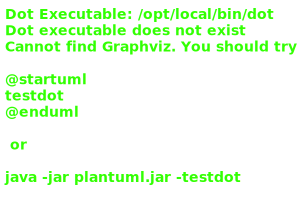
\includegraphics[width=0.9\textwidth]{../diagrams/system-context.png}
  \caption{AdvanDEB System Context}
  \label{fig:system-context}
\end{figure}

\section{Knowledge Builder}

The AdvanDEB Knowledge Builder is a FastAPI + Vue application used to construct and explore a biological knowledge base.

Figure~\ref{fig:kb-container} shows the main containers.
 
\begin{figure}[h]
  \centering
  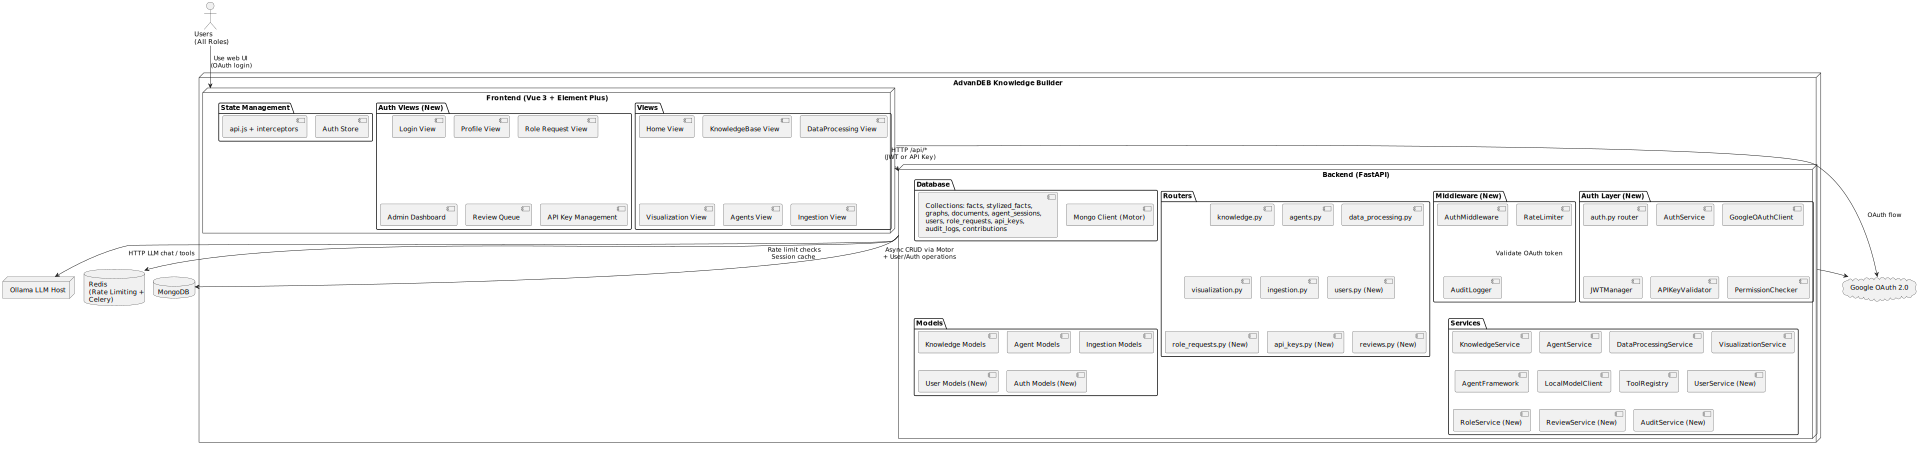
\includegraphics[width=0.9\textwidth]{../diagrams/knowledge-builder-container.png}
  \caption{Knowledge Builder Container Diagram}
  \label{fig:kb-container}
\end{figure}

\subsection{Data Model (Conceptual)}

Conceptually, the Knowledge Builder organises information into documents, facts, stylised facts, knowledge graph elements, and agent sessions. A high-level class diagram is shown in Figure~\ref{fig:kb-data-model}.

\begin{figure}[h]
  \centering
  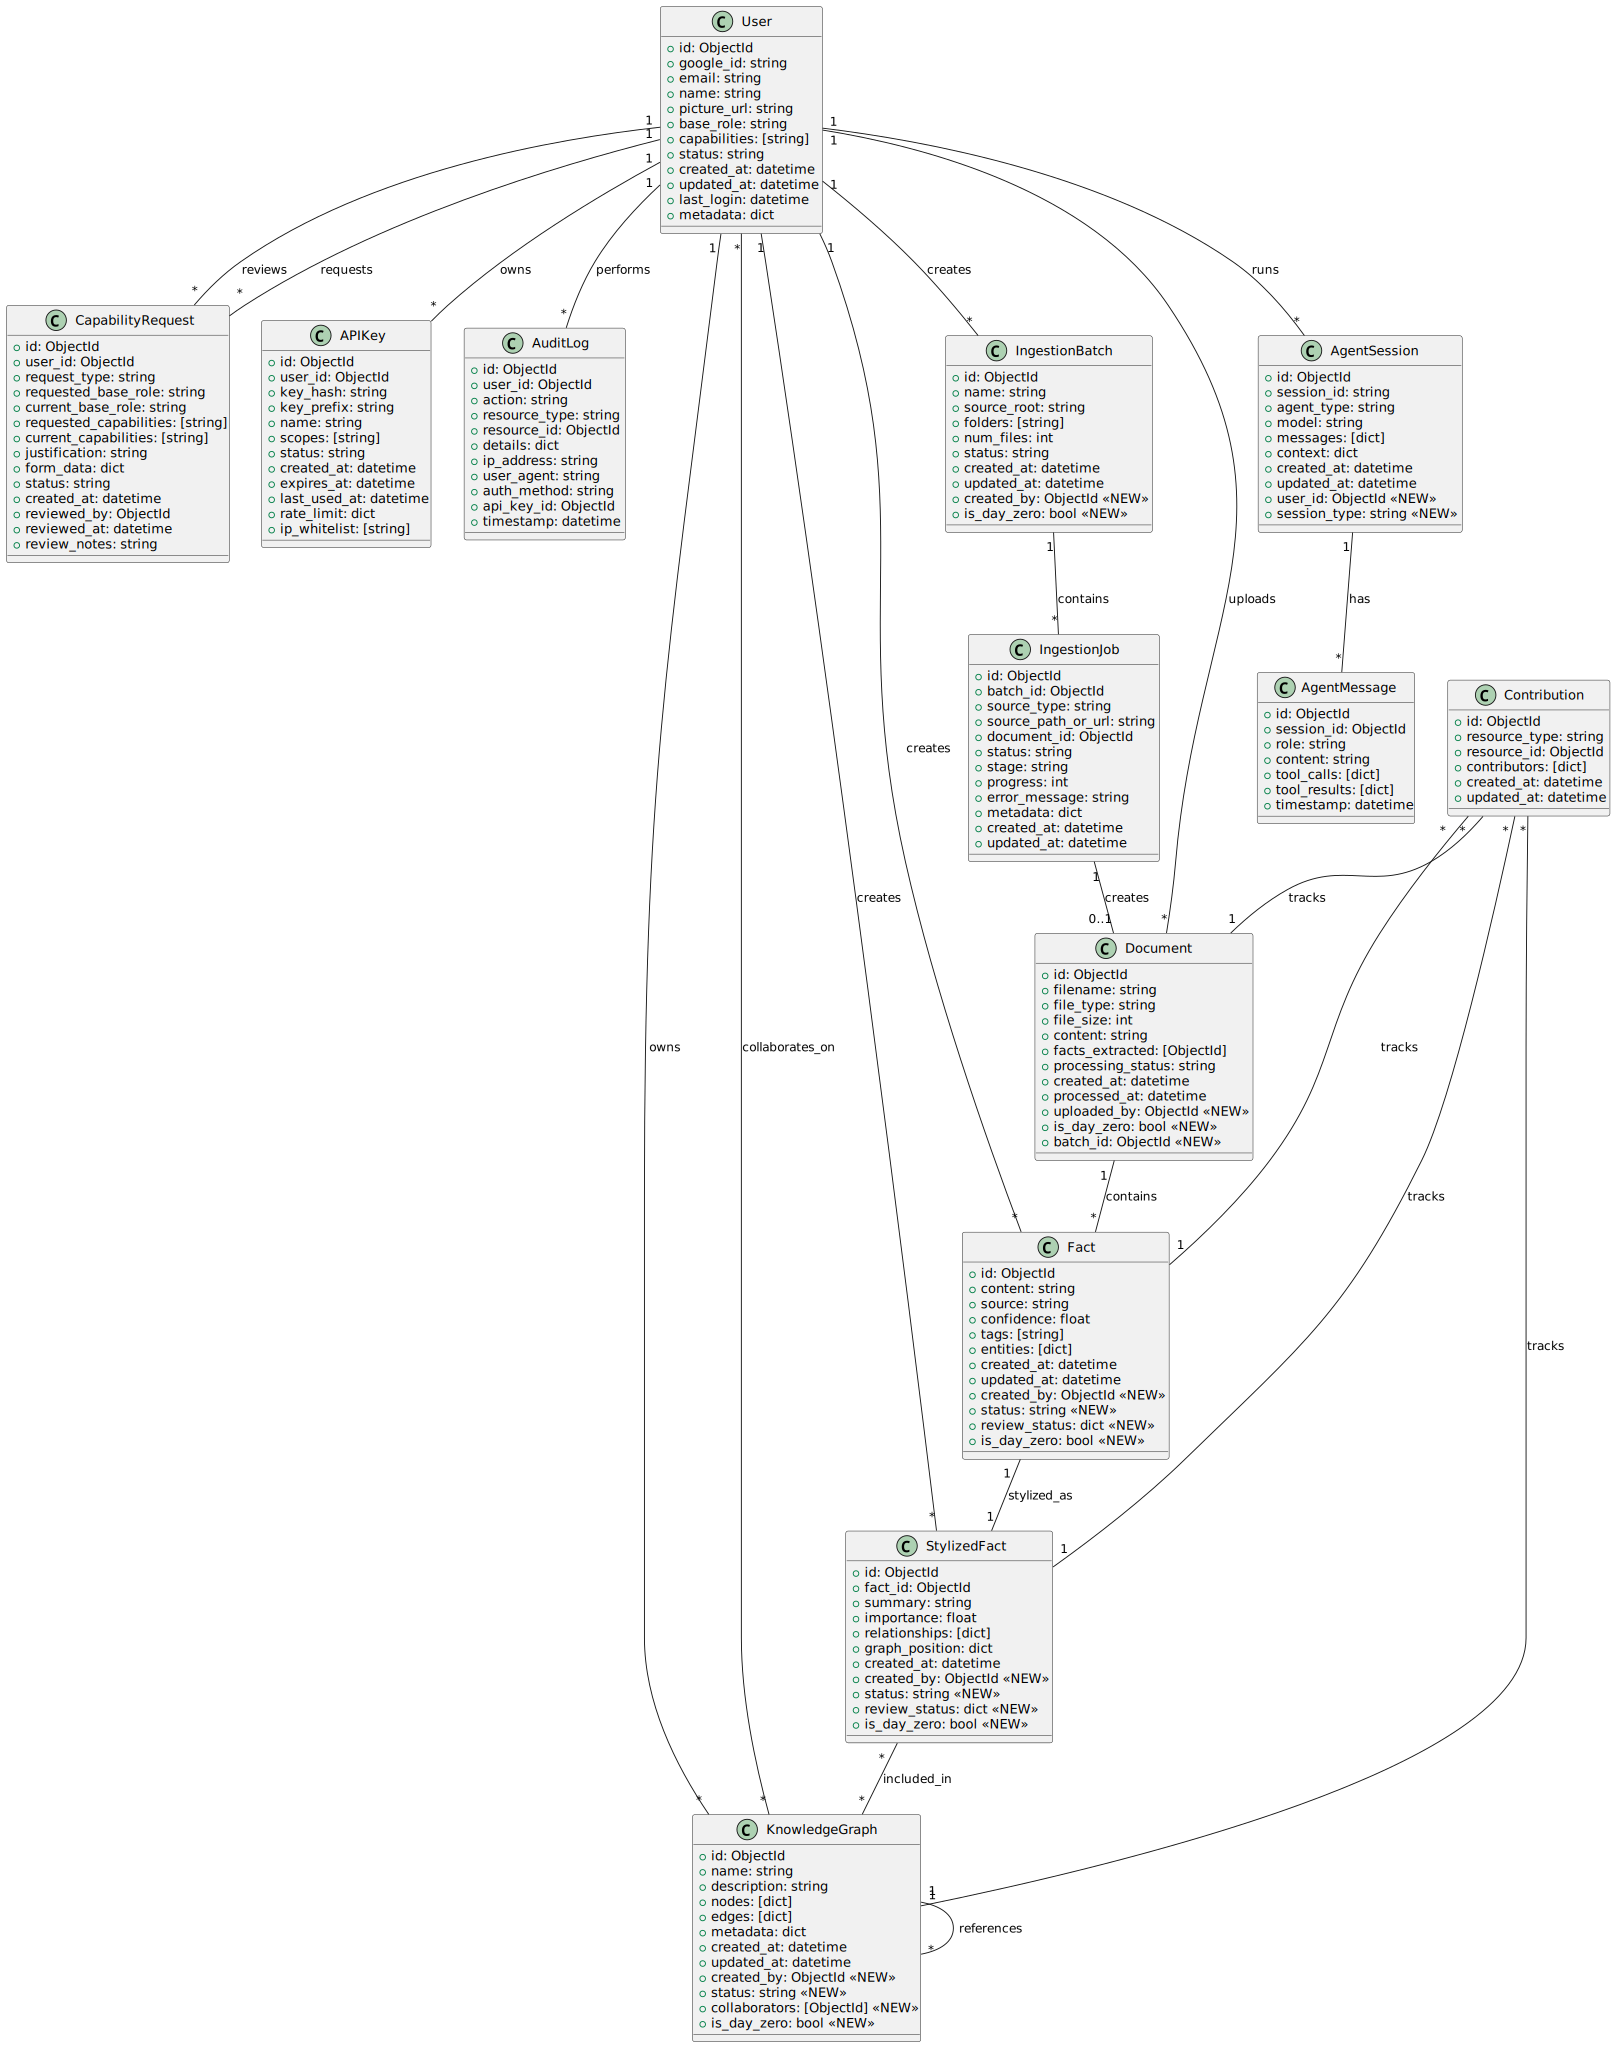
\includegraphics[width=0.9\textwidth]{../diagrams/knowledge-builder-data-model.png}
  \caption{Knowledge Builder Conceptual Data Model}
  \label{fig:kb-data-model}
\end{figure}
 
\subsection{Document Ingestion Flow}

The document ingestion and fact extraction sequence is illustrated in Figure~\ref{fig:doc-ingestion}.

\begin{figure}[h]
  \centering
  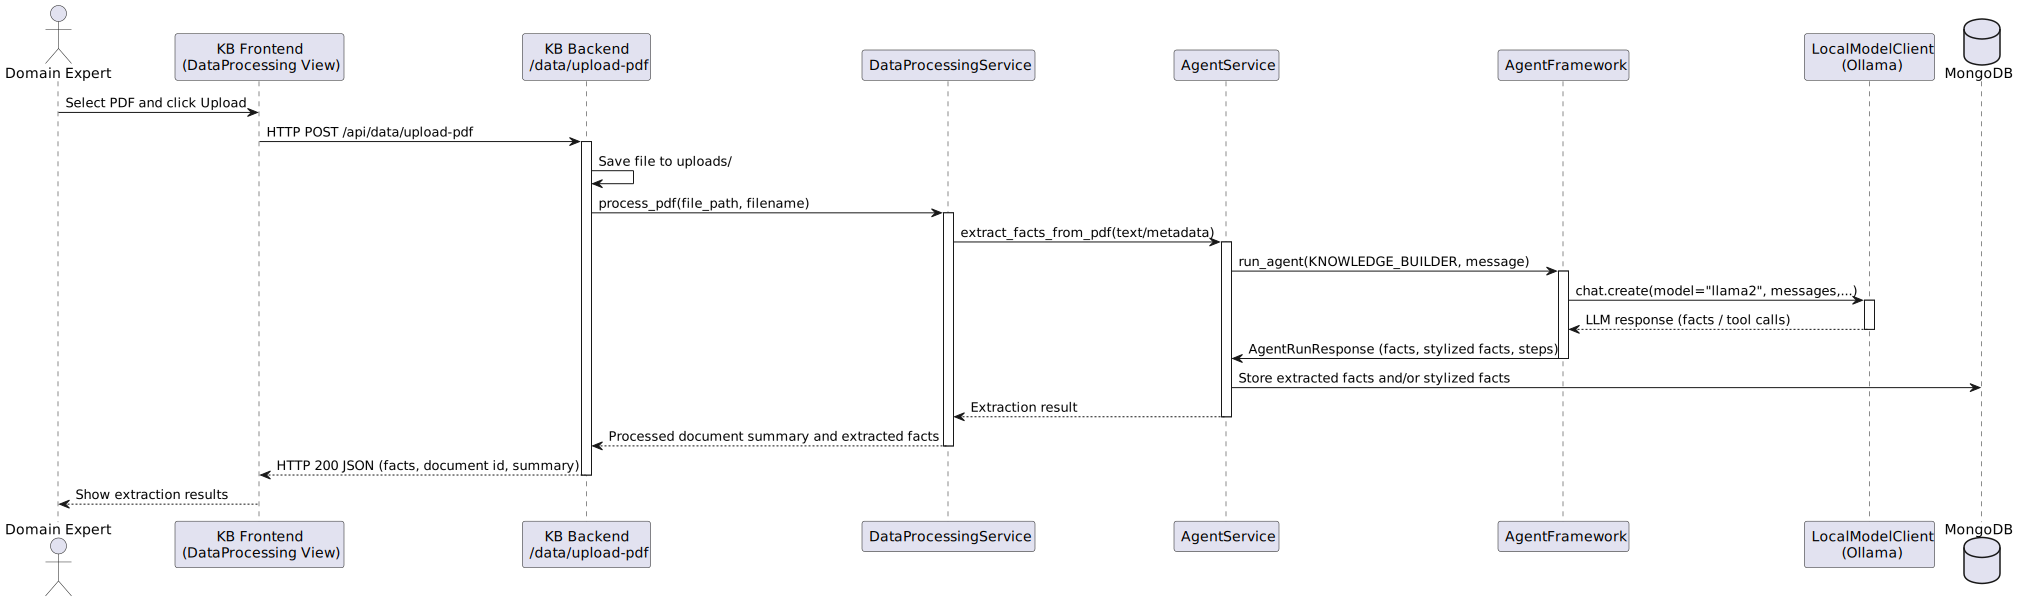
\includegraphics[width=0.9\textwidth]{../diagrams/document-ingestion-sequence.png}
  \caption{Document Ingestion and Fact Extraction}
  \label{fig:doc-ingestion}
\end{figure}

\section{Modeling Assistant}

The AdvanDEB Modeling Assistant is a planned component that will consume knowledge from the Knowledge Builder to support individual-based modeling.

Figure~\ref{fig:ma-container} shows its planned containers and dependencies.

\begin{figure}[h]
  \centering
  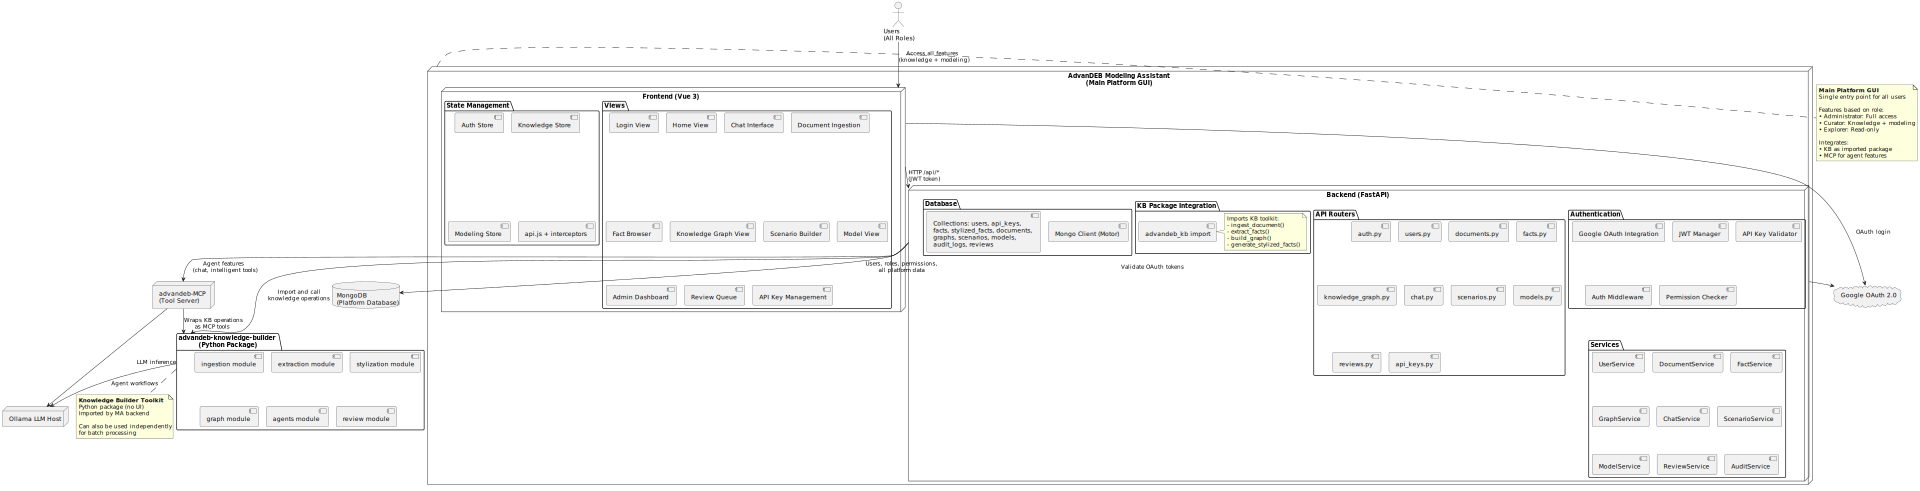
\includegraphics[width=0.9\textwidth]{../diagrams/modeling-assistant-container.png}
  \caption{Modeling Assistant Container Diagram (Planned)}
  \label{fig:ma-container}
\end{figure}

\section{Development Environment}

All services use a single Conda environment named \texttt{advandeb}. The canonical \texttt{environment.yml} is stored in the \texttt{advandeb-architecture} repository.

To create and activate the environment:

\begin{verbatim}
conda env create -f environment.yml
conda activate advandeb
\end{verbatim}

Core external services:

\begin{itemize}[noitemsep]
  \item MongoDB (default: \texttt{mongodb://localhost:27017})
  \item Ollama (default: \texttt{http://localhost:11434})
\end{itemize}

\section{Integration APIs}

The Modeling Assistant interacts with the Knowledge Builder primarily via HTTP APIs. This section summarises the main contracts; full details are maintained in the Markdown documentation (e.g., \texttt{docs/markdown/INTEGRATION-APIS.md}).

\subsection{Knowledge Search}

The Knowledge Builder exposes an endpoint for free-text search over facts, stylised facts, and graph elements.

\begin{itemize}[noitemsep]
  \item Endpoint: \texttt{GET /api/knowledge/search}
  \item Typical parameters: query string \texttt{q}, optional type filter (e.g., \texttt{fact}, \texttt{stylized\_fact}, or \texttt{graph\_node}), and a result limit.
  \item Response: a list of scored results with identifiers, text, source references, and tags.
\end{itemize}

\subsection{Facts and Stylised Facts}

Individual facts and stylised facts can be retrieved by identifier.

\begin{itemize}[noitemsep]
  \item Endpoint: \texttt{GET /api/knowledge/facts/\{fact\_id\}}
  \item Endpoint: \texttt{GET /api/knowledge/stylized-facts/\{stylized\_fact\_id\}}
  \item Responses include text, source, timestamps, tags, and optional metadata.
\end{itemize}

\subsection{Graph Exploration}

To understand local structure around entities, the Modeling Assistant can request graph neighbourhoods.

\begin{itemize}[noitemsep]
  \item Endpoint: \texttt{GET /api/knowledge/graph/neighborhood}
  \item Typical parameters: \texttt{node\_id}, a depth parameter, and a maximum number of nodes.
  \item Response: sets of nodes and edges that can be visualised or analysed.
\end{itemize}

\subsection{Agent Invocation}

The Knowledge Builder also provides higher-level reasoning via agents.

\begin{itemize}[noitemsep]
  \item Endpoint: \texttt{POST /api/agents/run}
  \item Request: an agent identifier, natural-language input, and an optional context referencing facts, stylised facts, or graph nodes.
  \item Response: structured or textual output from the agent, tool call traces, and a session identifier for follow-up interactions.
\end{itemize}

\subsection{Modeling Assistant APIs}

The Modeling Assistant exposes its own APIs for clients, while internally consuming the Knowledge Builder endpoints.

\begin{itemize}[noitemsep]
  \item Scenario management (e.g., \texttt{POST /api/scenarios}) to define modelling problems and objectives.
  \item Model proposal endpoints (e.g., \texttt{POST /api/scenarios/\{scenario\_id\}/propose-model}) that assemble candidate model structures and provide justifications referencing Knowledge Builder items.
\end{itemize}

\section{Future Work}

Planned extensions to this printable document include:

\begin{itemize}[noitemsep]
  \item Detailed data model diagrams for the Knowledge Builder.
  \item Additional sequence diagrams for Modeling Assistant workflows.
  \item Short design decision records for major architectural choices.
\end{itemize}

\end{document}
